\ssr{Введение}

Цели данной лабораторной работы:
\begin{enumerate}
	\item изучить основные команды и инструменты для управления процессами;
	\item ознакомиться со средствами мониторинга производительности в Linux;
	\item приобрести практический навык автоматизации запуска процессов.
\end{enumerate}

\ssr{Выполнение}

\section{Мониторинг производительности системы}

\begin{figure}[!htbp]
	\centering
	\includegraphics[width=0.6\linewidth]{"Screenshot From 2026-10-19 13-00-44.png"}
	\includegraphics[width=0.6\linewidth]{"Screenshot From 2026-10-19 13-02-54.png"}
	\caption{Проверка системы при помощи команды top}
\end{figure}
\FloatBarrier

\begin{figure}[!htbp]
	\centering
	\includegraphics[width=0.6\linewidth]{"Screenshot From 2026-10-19 13-04-20.png"}
	\caption{Изменение приоритета запущенного процесса командой renice}
\end{figure}
\FloatBarrier

\begin{figure}[!htbp]
	\centering
	%\includegraphics[width=0.6\linewidth]{}
	\caption{Cортировка процессов с помощью команд atop и atopsar}
\end{figure}
\FloatBarrier

\begin{figure}[!htbp]
	\centering
	\includegraphics[width=0.6\linewidth]{"Screenshot From 2026-10-19 13-36-46.png"}
	\includegraphics[width=0.6\linewidth]{"Screenshot From 2026-10-19 13-37-09.png"}
	\caption{Вывод информации по процессорам при помощи команды mpstat и опции P}
\end{figure}
\FloatBarrier

\begin{figure}[!htbp]
	\centering
	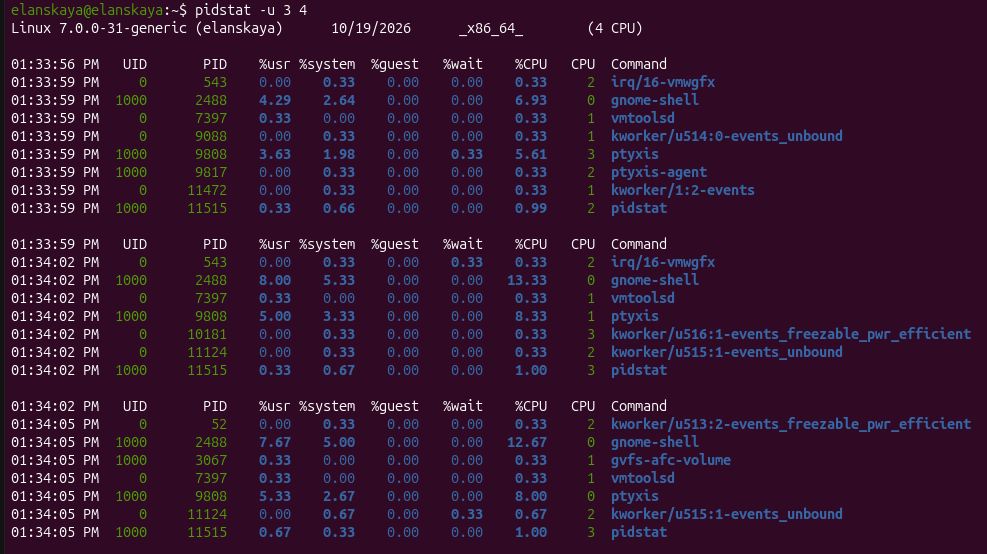
\includegraphics[width=0.6\linewidth]{Screenshot From 2026-10-19 13-37-29.png}
	\caption{Проверка системы при помощи команды pidstat}
\end{figure}
\FloatBarrier

\section{Создание скрипта для получения статистики}

Скрипт, осуществляющий сбор статистики использования процессоров и статистики работы процессов средствами mpstat и pidstat, выводящий данные в текстовый файл с именем yyyy-mm-dd\_h:m:s\_syslog, представлен в листинге~\ref{stat}.

\lstinputlisting[
	label={stat}, 
	style=bash, 
	caption={Код скрипта для сбора статистики}
]{statistics.sh}

%\lstinputlisting[style=text, caption={Файл лога}]{}

\begin{figure}[!htbp]
	\centering
	\includegraphics[width=0.6\linewidth]{"Screenshot From 2026-10-19 14-03-55.png"}
	\caption{Вывод команды ls -l для директории сохранения логов скрипта}
\end{figure}
\FloatBarrier

\section{Создание автозапускаемой службы}

Код файла службы по сбору статистики, запускающую скрипт из задания 2 при старте системы, представлен в листинге~\ref{service}.


\lstinputlisting[
	label={service},
	style=yaml, 
	caption={Служба для сбора статистики}
]{statistics.service}

\begin{figure}[!htbp]
	\centering
	%\includegraphics[width=0.6\linewidth]{"Screenshot From 2026-10-19 14-04-14.png"}
	\includegraphics[width=0.6\linewidth]{"Screenshot From 2026-10-19 14-04-34.png"}
	\caption{Вывод команды ls -l для директории сохранения логов скрипта}
\end{figure}
\FloatBarrier

\ssection{Дополнительное задание}

%\lstinputlisting[style=bash, caption={Код таймера для запуска каждую минуту}]{}

Результаты работы таймера для службы из задания 3 представлены в листинге~\ref{timer} и на рисунке~\ref{timer:log}

\lstinputlisting[
	label={timer}, 
	style=yaml, 
	caption={Юнит таймера}
]{statistics.timer}

\begin{figure}[!htbp]
	\centering
	\includegraphics[width=0.6\linewidth]{"Screenshot From 2026-10-19 14-05-32.png"}
	\caption{Результат работы таймера}
	\label{timer:log}
\end{figure}
\FloatBarrier

\ssr{Вывод}

В ходе лабораторной работы: 
\begin{itemize}
	\item были изучены основные команды и инструменты для управления процессами;
	\item было проведено ознакомление со средствами мониторинга производительности в Linux;
	\item был приобретен практический навык автоматизации запуска процессов.
\end{itemize}

\ssr{Контрольные вопросы}

\begin{enumerate}
	\item \textit{Дайте определение процессу, программе. }\newline 
	Процесс -- это программа в стадии выполнения или, с точки зрения операционной системы, сущность, представляющая понятие активности/работы. Процесс обладает уникальным идентификатором (PID) и контекстом выполнения (стек вызовов, снимок регистров процессора и др.), необходимым для корректной работы в многозадачной системе.
	Программа -- файл, содержащий исполняемый код (машинные инструкции) и данные, хранящийся на носителе.
	\item \textit{Какие утилиты позволяют отобразить информацию о работающих процессах? Как еще можно получить информацию о процессах в ОС -- приведите пример }\newline 
	Утилиты ps, top, atop, pidstat, а также atopsar (анализ логов atop), mpstat, vmstat, iostat (пакет sysstat).
	Пример: 
	\begin{itemize}
		\item ps aux -- вывод всех процессов с потреблением CPU и памяти;
		\item pgrep -a <name> -- поиск процессов по имени с аргументами командной строки;
		\item ps -p PID -o pid,comm,\%cpu,\%mem -- информация по конкретному процессу;
		\item cat /proc/PID/status -- сведения о процессе из файловой системы procfs.
	\end{itemize}
	\item \textit{Как можно, используя top, посмотреть показатели потребления ресурсов для конкретного процесса?}\newline 
	Найти процесс по PID и смотреть по остальным колонкам. Удобнее использовать встроенный фильтр: нажать o и ввести условие (например, PID=<pid> или COMMAND=<name>) -- останется только нужная строка. Показатели: \%CPU, \%MEM, RES (резидентная память), VIRT, TIME+, NI (nice) и др.
	\item \textit{Что показывает команда systemctl status для службы, если получен статус active (exited)? Какие еще статусы могут быть?}\newline 
	Что служба отработала и корректно завершилась с кодом 0. 
	Другие статусы: active (running), inactive (dead), failed, activating, deactivating, reloading, active (waiting) для таймеров.
	\item \textit{Если в секции Unit службы указывается After=network.target, гарантирует ли это наличие сетевого подключения?}\newline
	Нет. After=network.target задает только порядок запуска (после network.target), но не гарантирует наличие сетевого подключения. Для зависимости от сети используют network-online.target
	\item \textit{От имени какого пользователя по умолчанию будет запускаться служба?}\newline 
	От root.
	\item \textit{Как указать конкретного пользователя, от имени которого будет запускаться служба? Каких проблем позволяет избежать явное указание пользователя?}\newline 
	В секции [Service] указать User=<name> (при необходимости -- \\ Group=<name>). 
	Снижает риски, так как служба не получит избыточных прав.
	\item \textit{Что означает указание типа службы Type=simple? Какой тип нужно указывать в случае, если служба должна работать постоянно?}\newline 
	Процесс запускается сразу, systemd считает службу запущенной без ожидания готовности (процесс не форкается).
	Для постоянно работающей службы -- Type=simple (процесс не завершается), для форкающихся -- Type=forking.
	\item \textit{Как называется постоянно работающая фоновая служба? Приведите пример такой службы, используемой вами }\newline 
	Демон (daemon). 
	Пример: crond, snapd, systemd-journald (буква d на конце -- обычно индикатор демона).
	\item \textit{В файл загруженной ранее и успешно отработавшей службы \\ my\_service.service внесены изменения. Достаточно ли для их применения использовать команду systemctl restart my\_service.service?}\newline 
	Нет, недостаточно. После правки юнита нужен sudo systemctl daemon-reload, затем sudo systemctl restart my\_service.service.
	\item \textit{Вам нужно проанализировать возможные проблемы производительности системы по запросу – например, поступила информация, что система «тормозила» около 16:00 вчера. Вы предполагаете, что проблема может быть вызвана нехваткой RAM. Какой командой имеет смысл воспользоваться для диагностики?}\newline 
	Командой atopsar -m -b 15:50:00 -e 16:10:00 -r /var/log/atop/atop\_YYYYMMDD (анализ нагрузки на RAM за период). 
	При наличии sysstat также sar -r -s 15:50:00 -e 16:10:00. Дополнительно полезны sar -B (paging/swapping) и atopsar -m для оценки нехватки памяти.
\end{enumerate}
